%=========================================================================
% SM 11/2016
% Mid Term Report IISER Thiruvananthapuram
% Chapter 3
%=========================================================================

\chapter{SNR and Overlap Study of SpinTaylorF2}

In this chapter we investigate how the signal-to-noise ratio of the full
SpinTaylorF2 waveform for a generic NSBH binary varies over extrinsic $(\theta_J,
\psi_J)$ and $(\chi_1, \kappa, \eta)$ intrinsic parameters. We find that precession
as well as the orientation of the binary in the sky have an observable imprint 
on the SNR variation of the full waveform across the spin-precession $(\theta_J,
\kappa)$ parameter space. We then investigate how the total SNR is
distributed among the individual sidebands by computing the overlap of the
sideband with the full waveform, in the exact same regions of the 
spin-precession parameter space.

\section{Definitions of SNR and overlap}

The characteristic signal-to-noise ratio (SNR) of a frequency domain waveform
$h(f)$ is given by $(h|h)$, where $(a|b)$ is the noise-weighted scalar product
defined as
\label{inner_product}  
\begin{equation} (a|b) = 4 \text{Re} \left[
\int_{f_{1}}^{f_{2}}  \dfrac{a^{*}(f)b(f)}{S_{n}(f)} df\right].
\end{equation}
In the above equation $S_{n}(f)$ is the one-sided noise power spectral density
(PSD) of the detector~\cite{PSD}, and $a^{*}(f)$ is the complex conjugate of
the frequency domain waveform amplitude $a(f)$. The SNR---as the name
suggests---indicates how \textit{loud} the GW signal is compared to the
background noise of the detector. 

However, given the mathematical construction of the SpinTaylorF2 waveform, we
are more interested in the fractional SNR contribution by the sidebands to the
total SNR of the SpinTaylorF2 waveform. To do this, we compute the overlap of
each of the sidebands with the full waveform. The overlap between two
frequency domain amplitudes $a(f)$ and $b(f)$ is defined as
(see~\cite{Lundgren2014}):
\begin{equation} 
O_{ab} \equiv \dfrac{(a|b)}{\sqrt{(a|a)(b|b)}},
\end{equation} 
where $(a|b)$ is the noise-weighted inner product defined in
Eq.~(\ref{inner_product}). For our analyses, we define the overlap of the
$m^{\rm th}$ sideband with the full waveform as:
\begin{equation} 
O_{m} \equiv \dfrac{(h_m|h)}{\sqrt{(h_m|h_m)(h|h)}},
\end{equation} 
where $h_m$ corresponds to the $m^{\rm th}$ sideband, and $h$ represents the
full SpinTaylorF2 waveform. Note that the overlap function is normalized, and
is equal to zero if the waveforms are `orthogonal' to each other, and equal to
one, if they are exactly equal.

\section{SNR study in the $(\theta_J, \kappa)$ parameter space}

We computed the variation of SNR of full SpinTaylorF2 waveform in the
$(\theta_J, \kappa)$  space, for NSBH binaries with different $\chi_1$ and
$\eta$ values. We fixed the neutron star mass $(m_{2})$ to $1.4\,M_{\odot}$,
in agreement with the NS mass distribution in observed BNS systems reported
by~\cite{Lorimer}. Fig.~(\ref{fig:SNR}) shows the variation SNR of the
SpinTaylorF2 waveform over $(\theta_J, \kappa)$ the parameter space, for
different $\chi$ and $\eta$ values. We considered three BH masses
$m_1=2M_\odot, ~8M_\odot$ and $14 M_\odot$ (or equivalently $\eta = 0.24,
0.13$ and $0.08$) and two spin magnitudes  $\chi_1 = 0.5$ and $0.8$, and
constructed a $(2\times 3)$ panel, where the BH mass increases along each
column (top to bottom), and BH spin increases along each row (left to right).
For all the simulations, the source distance was fixed at $D=400$~Mpc.

\begin{figure}[t]
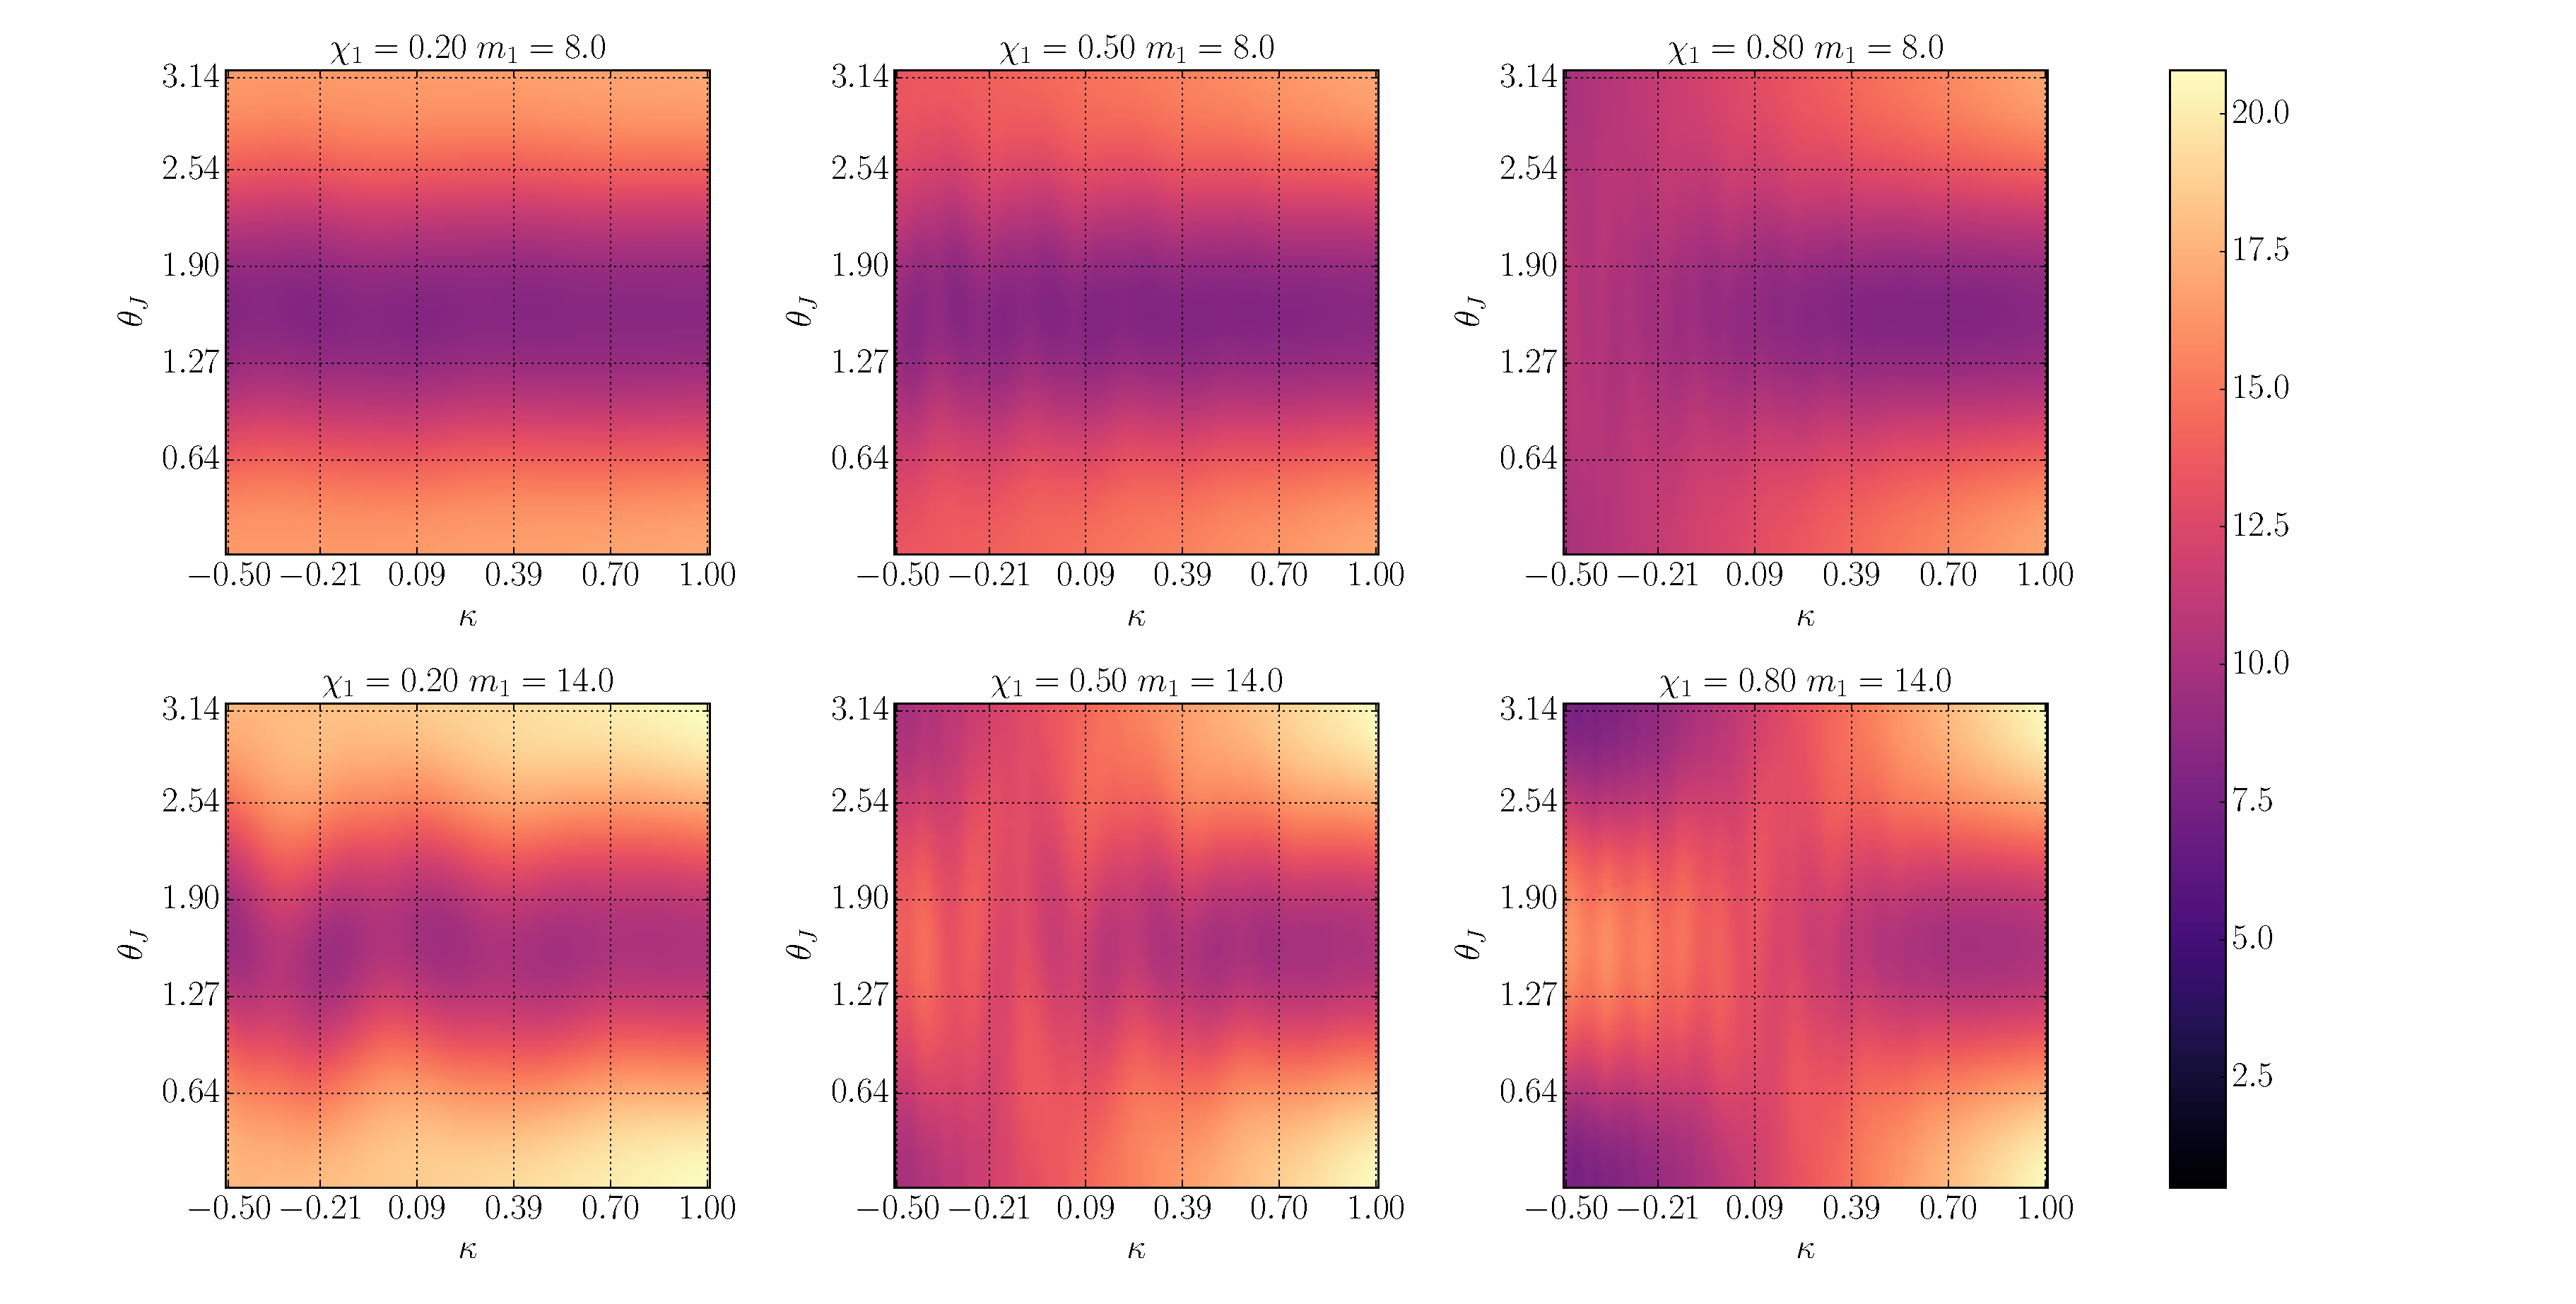
\includegraphics[width=\textwidth]{images/SNR_0F.pdf}
\caption{Variation of SNR in the $(\theta_J, \kappa)$ parameter space for 
different $\chi$ and $\eta$ values, where $\chi$ changes over the horizontal 
axis of the grid and $\eta$ varies over the vertical axis of the grid.}
\centering 
\label{fig:SNR} 
\end{figure}

We observe that the maximum SNR increases with the increasing BH mass (i.e.
lower $\eta$). Further, for non-precessing systems (top right panel, with
$m=14 M_\odot$ and $\chi_1=0.2$), the SNR is the highest in the face-on and
face-off regions $(\theta_{J} = 0/\pi)$. This represents a typical SNR map for
non-precessing systems, where the observed SNR of the signal only depends on
orientation of the binary in the sky. However, for a strongly precessing
system, i.e, with high mass asymmetry and high BH spin (bottom row, extreme
right panel), the SNR pattern shows variation over the spin-alignment
parameter $\kappa$. For $\kappa \sim 1$, the system is essentially a non-
precessing system and shows similar features (SNR is maximum in the face-on
and face-off regions) as discussed before. However, for $\kappa < 0$, the
system is strongly precessing and for these values of $\kappa$ the SNR pattern
is reversed, and the SNR is maximum near the edge-on regions.

All of these features can be explained by comparing the results with
expression for the frequency independent part of waveform amplitude in the
presence of precession; see Eq.~(A4) in~\cite{Apostolatos1994}:
\label{amplitudes}
\begin{equation}
H_{+} = \frac{1}{2}\frac{4 m_{1}m_{2}}{rD} \left[1 + (\hat{\mathbf{L}}\cdot\hat{\mathbf{N}})^{2}\right], 
H_{\times} = \frac{4 m_{1}m_{2}}{rD}\left[\hat{\mathbf{L}}\cdot\hat{\mathbf{N}}\right].
\end{equation}
The above equation suggests that the SNR---which is directly proportional to
the square of the  amplitude of the waveform---increases with increasing mass,
and that the amplitudes are maximum when $\mathbf{L}$ is along the line of
sight $\hat{\mathbf{N}}$. The second condition is precisely what the
combination of $(\theta_J, \kappa)$ satisfies, in regions where
the SNR peaks in the spin-precession parameter space.

Thus, Fig.~\ref{fig:SNR} clearly demonstrates that precession leads to
observable consequences for asymmetric, highly-spinning systems. For $\kappa$
close to 1 (aligned spin), the emission pattern is similar to non-precessing
systems (maximum SNR obtained for face-on or face-off cases). However, for
negative $\kappa$ values with anti-aligned spin (systems which show high
precession- induced modulations), the emission pattern is reversed (maximum
SNR for edge-on systems). In the intermediate region, however, the SNR results show an
interplay between the parameters $\kappa$ and $\theta_J$.

\section{Overlap study in the $(\theta_J, \kappa)$ parameter space}
We further computed the overlaps of all the sidebands $m=-2$ to $m=2$ with the
full SpinTaylorF2 waveform. We observed that the $m=0$ and  $m=2$ sidebands
are the dominant contributors to the total SNR of the full waveform over a
large region of the parameter space, except for a small region
$(\theta_J=0/\pi, \kappa \sim -0.5)$, where the $m=1$ seems to dominate.
However, since the total SNR in these regions is very low, we chose to study
the overlap variation of only the $m=0$ and  $m=2$ modes.

\label{fig:P2}  
\begin{figure}[!htp]
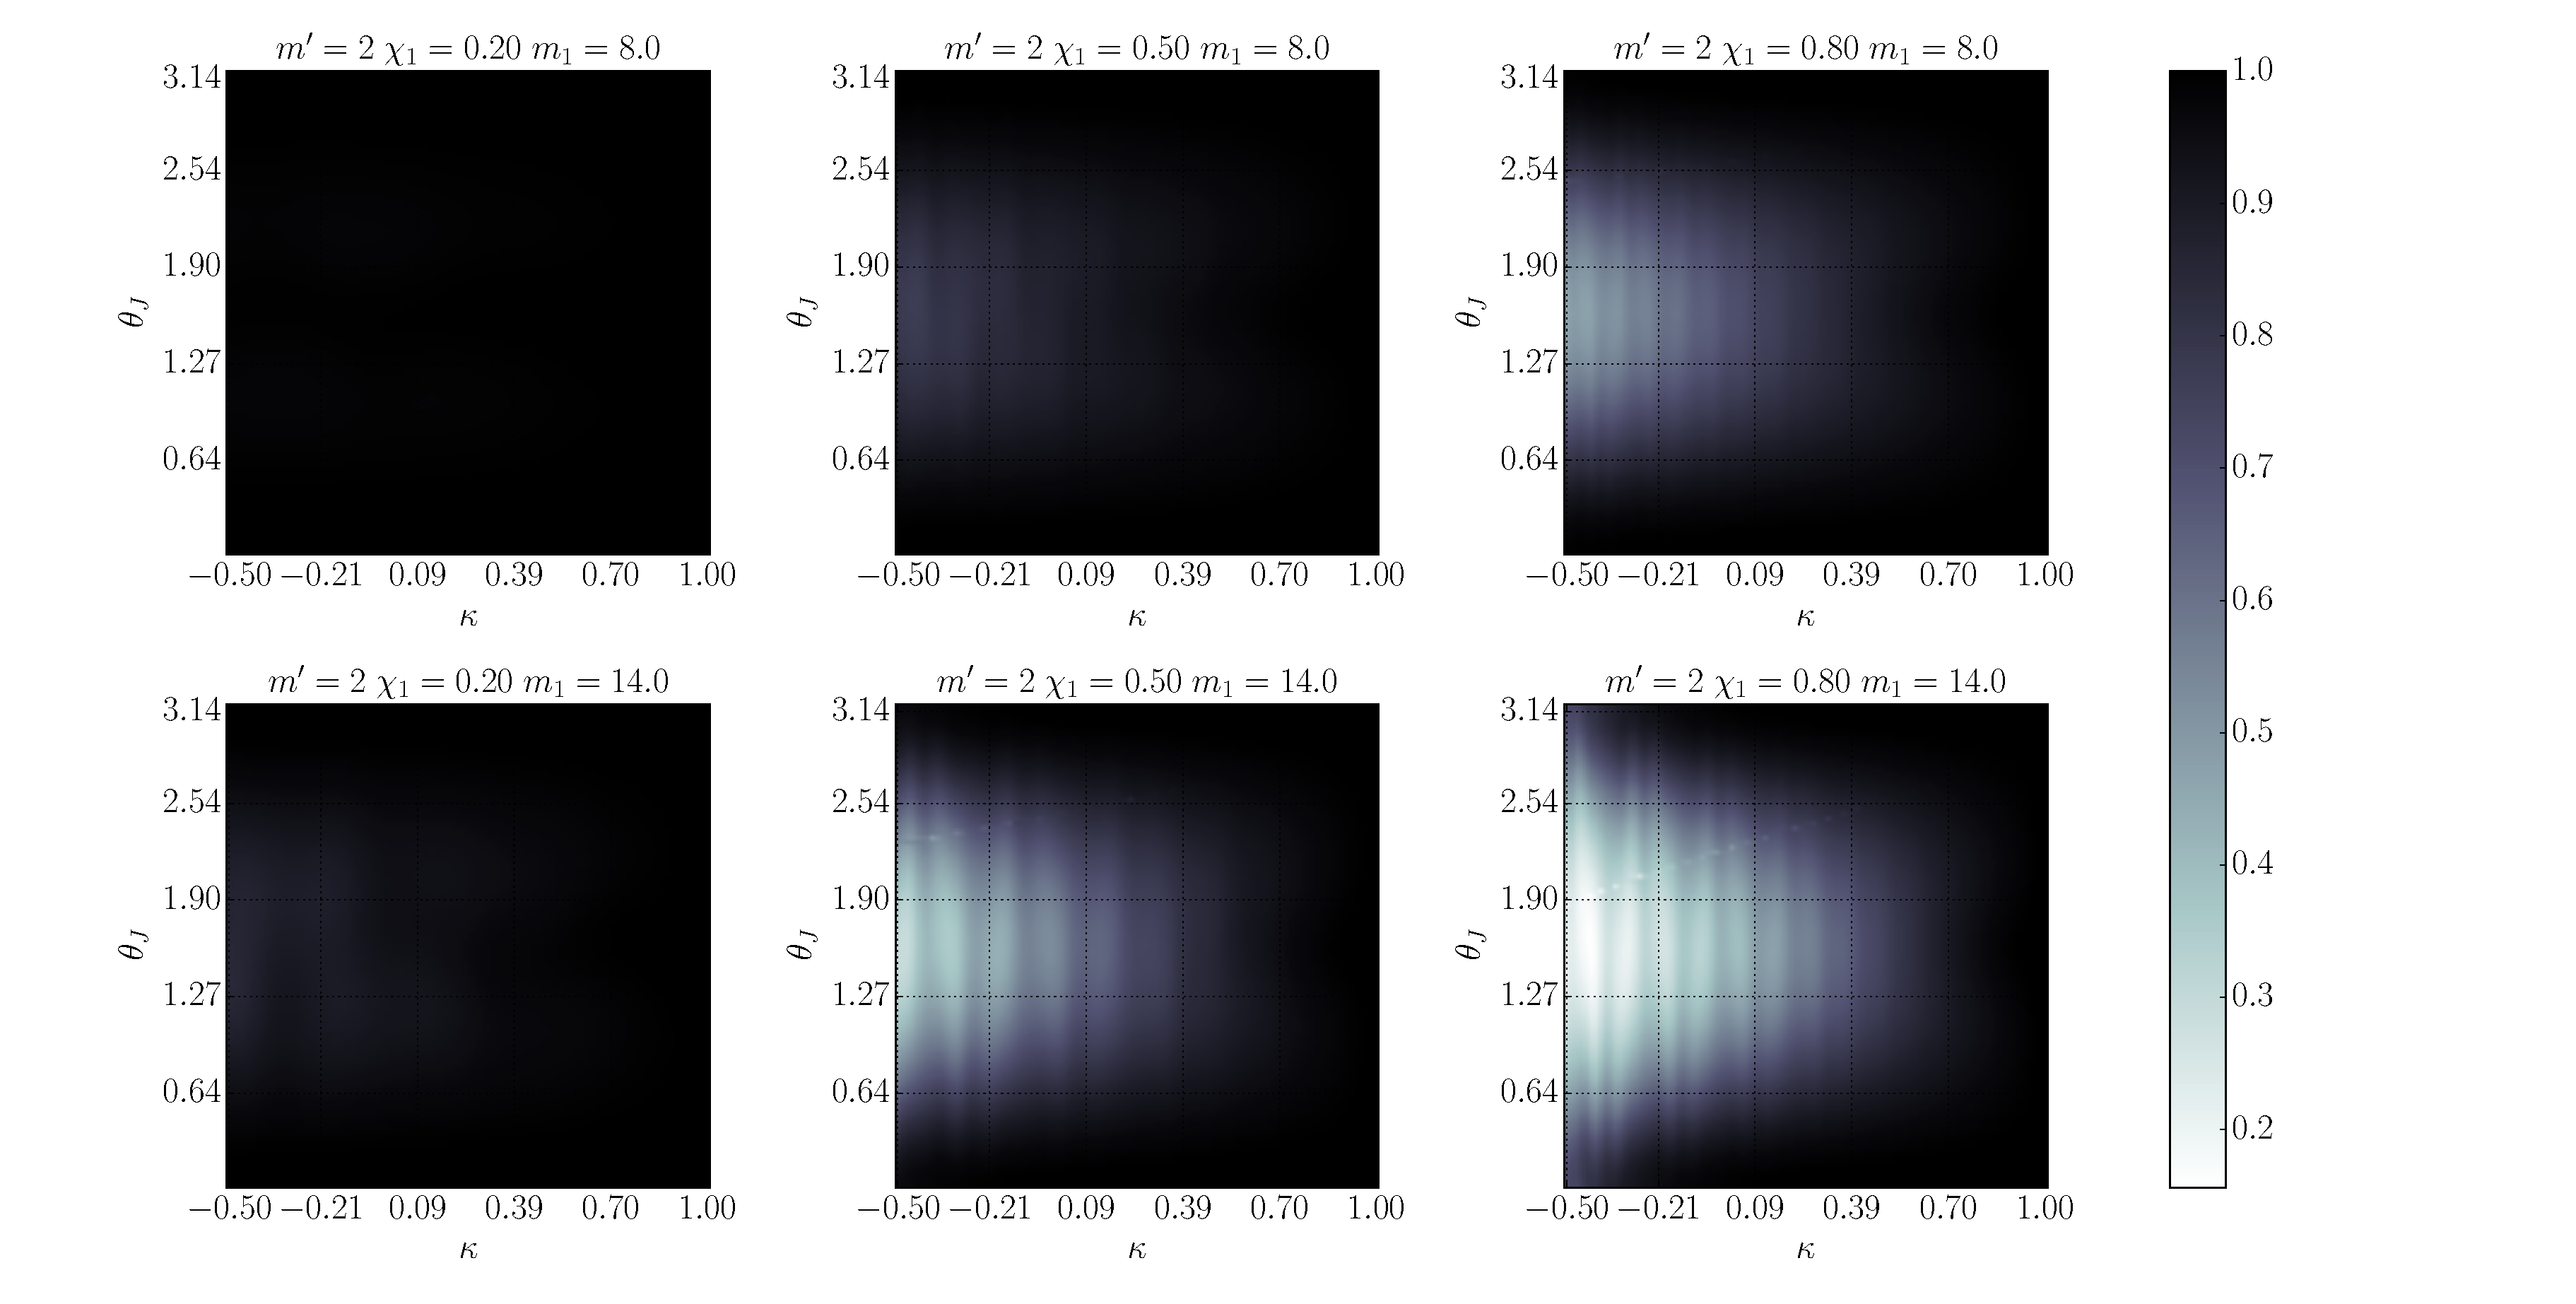
\includegraphics[width=\textwidth]{./images/OVLP_0F_P2.pdf}
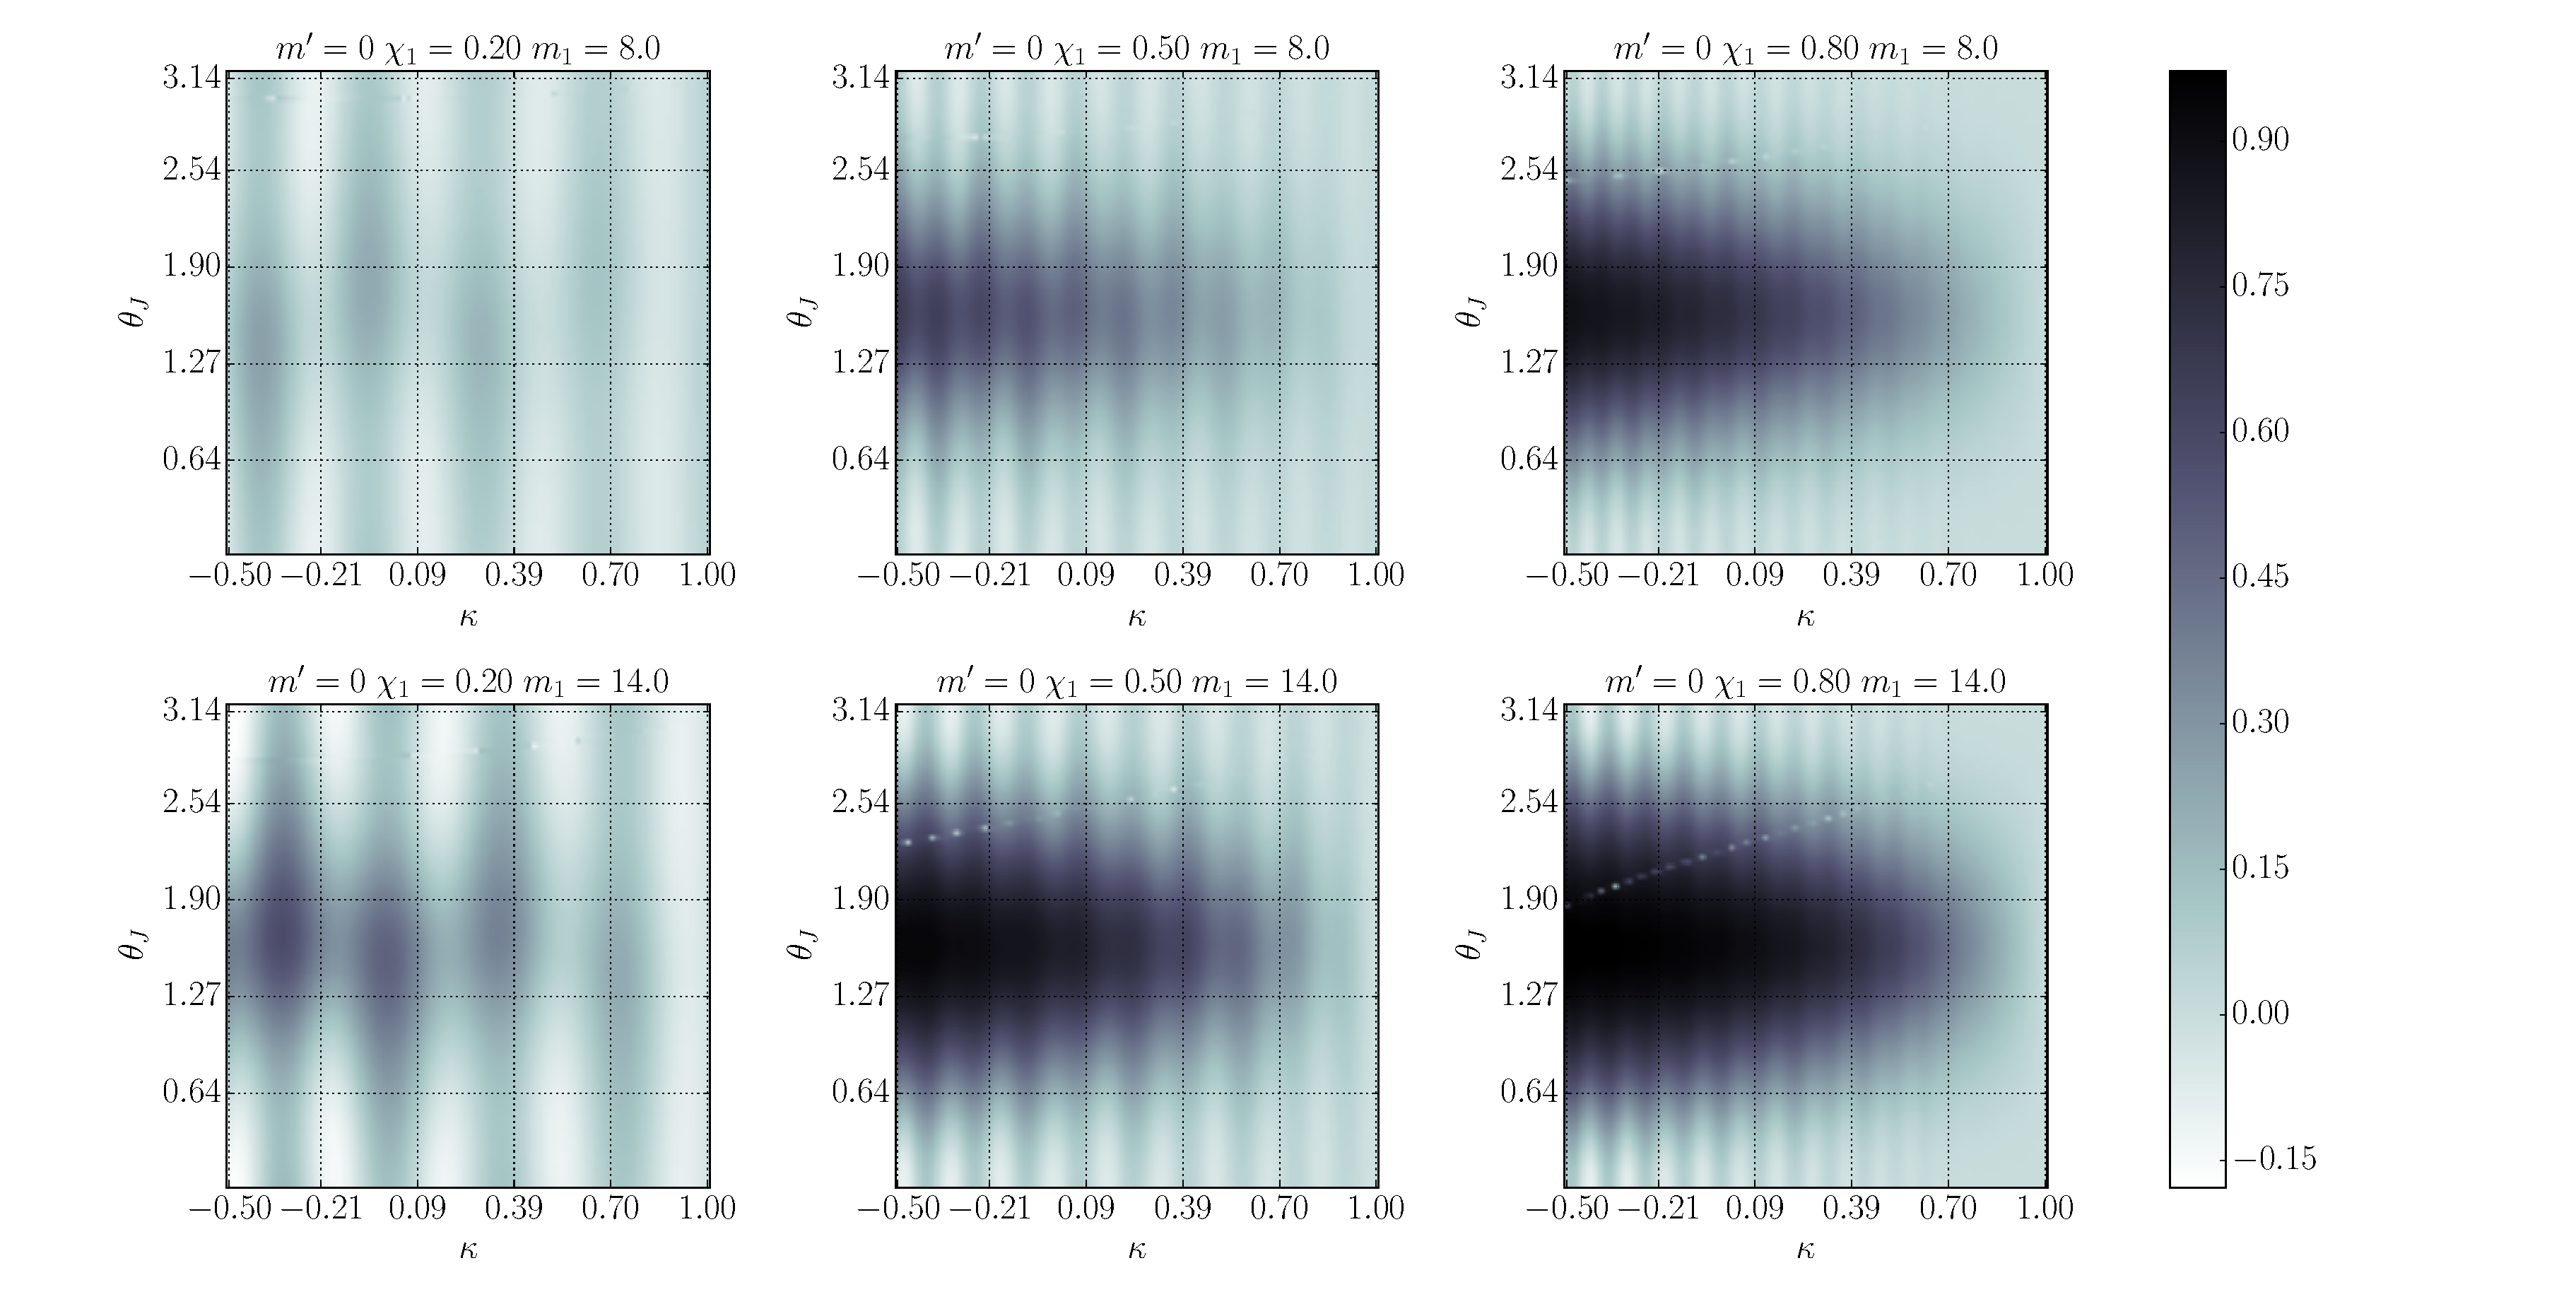
\includegraphics[width=\textwidth]{./images/OVLP_0F_P0.pdf} \caption{Variation
of overlap of $m=2$ and $m=0$ sideband with the SpinTaylorF2
waveform in the $(\theta_J, \kappa)$ parameter space for  different $\chi$ and
$\eta$ values, where $\chi$ changes over the horizontal axis of the grid and
$\eta$ varies over the vertical axis of the grid.}  
\centering  
\end{figure}

Similar to the SNR study, we investigated the variation of overlap the
$(\theta_J, \kappa)$ space using the exact same mass and spin parameters used
for studying the SNR variation. In Fig.~\ref{fig:P2}, we summarize our results
in two $(2 \times 3)$ panels, for $m=2$ and $m=0$ sidebands, respectively. We
must point out that regions of high overlap correspond to regions where there
is high fractional contribution of the sideband to the total SNR.

We immediately observe that the two maps of ${\cal{O}}_2$ and ${\cal{O}}_0$
exhibit strongly complementary features which indicate that the total SNR is
divided into these two dominant modes. Concretely, if the
system is highly precessing, most of the SNR is captured by the $m=0$
sideband, whereas if the system is mildly precessing the $m=2$ has the
dominant contribution to the SNR of the signal.  

Concretely, the $m=2$ mode appears to dominate (${\cal O}_2 \gg {\cal O}_0$)
for binaries with low mass-asymmetry (top row), or asymmetric mass binaries
with low-spin (left column). As the BH mass and spin increases, i.e., approach
towards strongly precessing systems, $m=2$ mode is dominant only for regions
where $\kappa \sim 1$, which are essentially non (mildly)-precessing systems.
In contrast, the $(m=0)$ mode shows high overlap (${\cal O}_0 \gg {\cal O}_2$)
near the edge-on region ($\theta_J=\pi/2$), and progressively covers more area
in the $(\theta_J, \kappa)$ space, as the spin or mass asymmetry increases,
i.e. for strongly precessing systems. In between, there exists be a region
where both for $m=2$ and $m=0$ sidebands contribute almost equally to the
total SNR (${\cal O}_2 \sim {\cal O}_0$), and we discuss this case in further
detail in the next chapter.


